\documentclass{standalone}
\usepackage{tikz}
\usetikzlibrary{arrows.meta}

\begin{document}

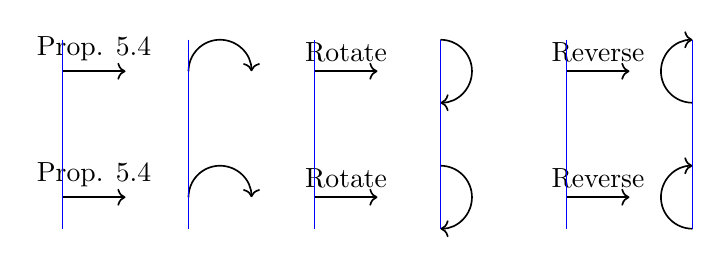
\begin{tikzpicture}[line width=0.6pt, scale=0.8]

% First Row
\draw[->] (0, 0) -- ++(1, 0) node[midway, above] {Prop. 5.4};
\draw[->] (2, 0) arc[start angle=180, end angle=0, radius=0.5];
\draw[->] (4, 0) -- ++(1, 0) node[midway, above] {Rotate};
\draw[->] (6, 0.5) arc[start angle=90, end angle=-90, radius=0.5];
\draw[->] (8, 0) -- ++(1, 0) node[midway, above] {Reverse};
\draw[->] (10, -0.5) arc[start angle=270, end angle=90, radius=0.5];

% Second Row
\draw[->] (0, -2) -- ++(1, 0) node[midway, above] {Prop. 5.4};
\draw[->] (2, -2) arc[start angle=180, end angle=0, radius=0.5];
\draw[->] (4, -2) -- ++(1, 0) node[midway, above] {Rotate};
\draw[->] (6, -1.5) arc[start angle=90, end angle=-90, radius=0.5];
\draw[->] (8, -2) -- ++(1, 0) node[midway, above] {Reverse};
\draw[->] (10, -2.5) arc[start angle=270, end angle=90, radius=0.5];

% Vertical Lines
\foreach \x in {0, 2, 4, 6, 8, 10} {
    \draw[blue] (\x, 0.5) -- (\x, -2.5);
}

\end{tikzpicture}

\end{document}